% fig-overlay-bus.tex
%
% Annotation overlay attached to the Hierarchy + Groupings core
% via a MolQL-style selector bus. Adopts the visual language of
% the post's other figures (palette, card styles, edge styles).
%
% The four grouping panels each show the SAME atom cloud with
% different lassos. Multiple labels per panel (D1/D2, R1/R2, ...)
% have visually distinct lasso styles. Some atoms are deliberately
% left unmapped in two of the panels to show that membership is
% sparse and not mandatory. Per-edge weights and operator details
% live in a side column rather than on the membership edges --
% this keeps the membership relation visually clean and treats the
% operator as the open-ended extension surface it is.

\documentclass[border=10pt,tikz]{standalone}
\usepackage{tikz}
\usepackage[T1]{fontenc}
\usepackage{lmodern}
\usepackage{amsmath, amssymb}
\usepackage{textcomp}
\usetikzlibrary{positioning, arrows.meta, fit, backgrounds, calc,
                shapes.geometric, decorations.pathreplacing}

% ---------- Unified palette (same as the other figures) ----------
\colorlet{H0}{black!16}
\colorlet{H1}{black!11}
\colorlet{H2}{black!7}
\colorlet{H3}{black!4}
\colorlet{H4}{black!1}
\colorlet{rule}{black!50}

\colorlet{accG}{teal!70!black}     % groupings
\colorlet{accO}{violet!70!black}   % operators
\colorlet{accS}{orange!75!black}   % R1
\colorlet{accT}{olive!65!black}    % R2
\colorlet{accA}{blue!55!black}     % annotations / selector bus

% ---------- Shared template ----------
\tikzset{
  card/.style    ={draw=rule, rounded corners=2pt, inner sep=4pt,
                   align=center, font=\sffamily\small, line width=0.5pt},
  L0/.style      ={card, fill=H0, minimum width=2.6cm},
  L1/.style      ={card, fill=H1, minimum width=2.2cm},
  L2/.style      ={card, fill=H2, minimum width=2.0cm},
  L3/.style      ={card, fill=H3, minimum width=1.7cm},
  L4/.style      ={card, fill=H4, minimum width=1.3cm,
                   font=\sffamily\footnotesize},
  more/.style    ={draw=rule!60, dashed, rounded corners=2pt, fill=white,
                   font=\sffamily\footnotesize\itshape, text=black!55,
                   minimum width=8mm, inner sep=2pt},
  Lanno/.style   ={card, fill=blue!3, draw=accA, line width=0.55pt,
                   minimum width=1.65cm, minimum height=8mm,
                   font=\sffamily\footnotesize},
  Lbus/.style    ={card, fill=blue!2, draw=accA, line width=0.7pt,
                   rounded corners=3pt, font=\sffamily\small},
  Lop/.style     ={card, fill=violet!4, draw=accO, line width=0.7pt,
                   minimum width=2.6cm, font=\sffamily\footnotesize,
                   align=left},
  panel/.style   ={card, fill=white, draw=rule!40, line width=0.4pt,
                   minimum width=3.2cm, minimum height=2.6cm,
                   inner sep=2pt},
  panelhdr/.style={font=\sffamily\footnotesize\bfseries, text=accG,
                   anchor=south},
  panelkind/.style={font=\sffamily\footnotesize\ttfamily, text=accG!85!black,
                    anchor=north},
  cloud-dot/.style={circle, fill=black!58, draw=none, inner sep=0pt,
                   minimum size=2.2pt},
  lasso-A/.style ={draw=accG, line width=0.7pt, rounded corners=2pt,
                   fill=teal!4, fill opacity=0.55},
  lasso-B/.style ={draw=accG, line width=0.7pt, dashed, rounded corners=2pt,
                   fill=teal!8, fill opacity=0.45},
  lasso-C/.style ={draw=accG, line width=0.7pt, dotted, rounded corners=2pt,
                   fill=teal!12, fill opacity=0.40},
  lassolbl/.style={font=\sffamily\tiny\ttfamily, text=accG!85!black,
                   inner sep=1pt, fill=white, fill opacity=0.85,
                   text opacity=1},
  contain/.style ={-, rule, line width=0.5pt},
  bind/.style    ={-Latex, accO, line width=0.7pt},
  annoWire/.style={-, accA, line width=0.45pt},
  busOut/.style  ={-Latex, accA, line width=0.9pt},
}

\begin{document}
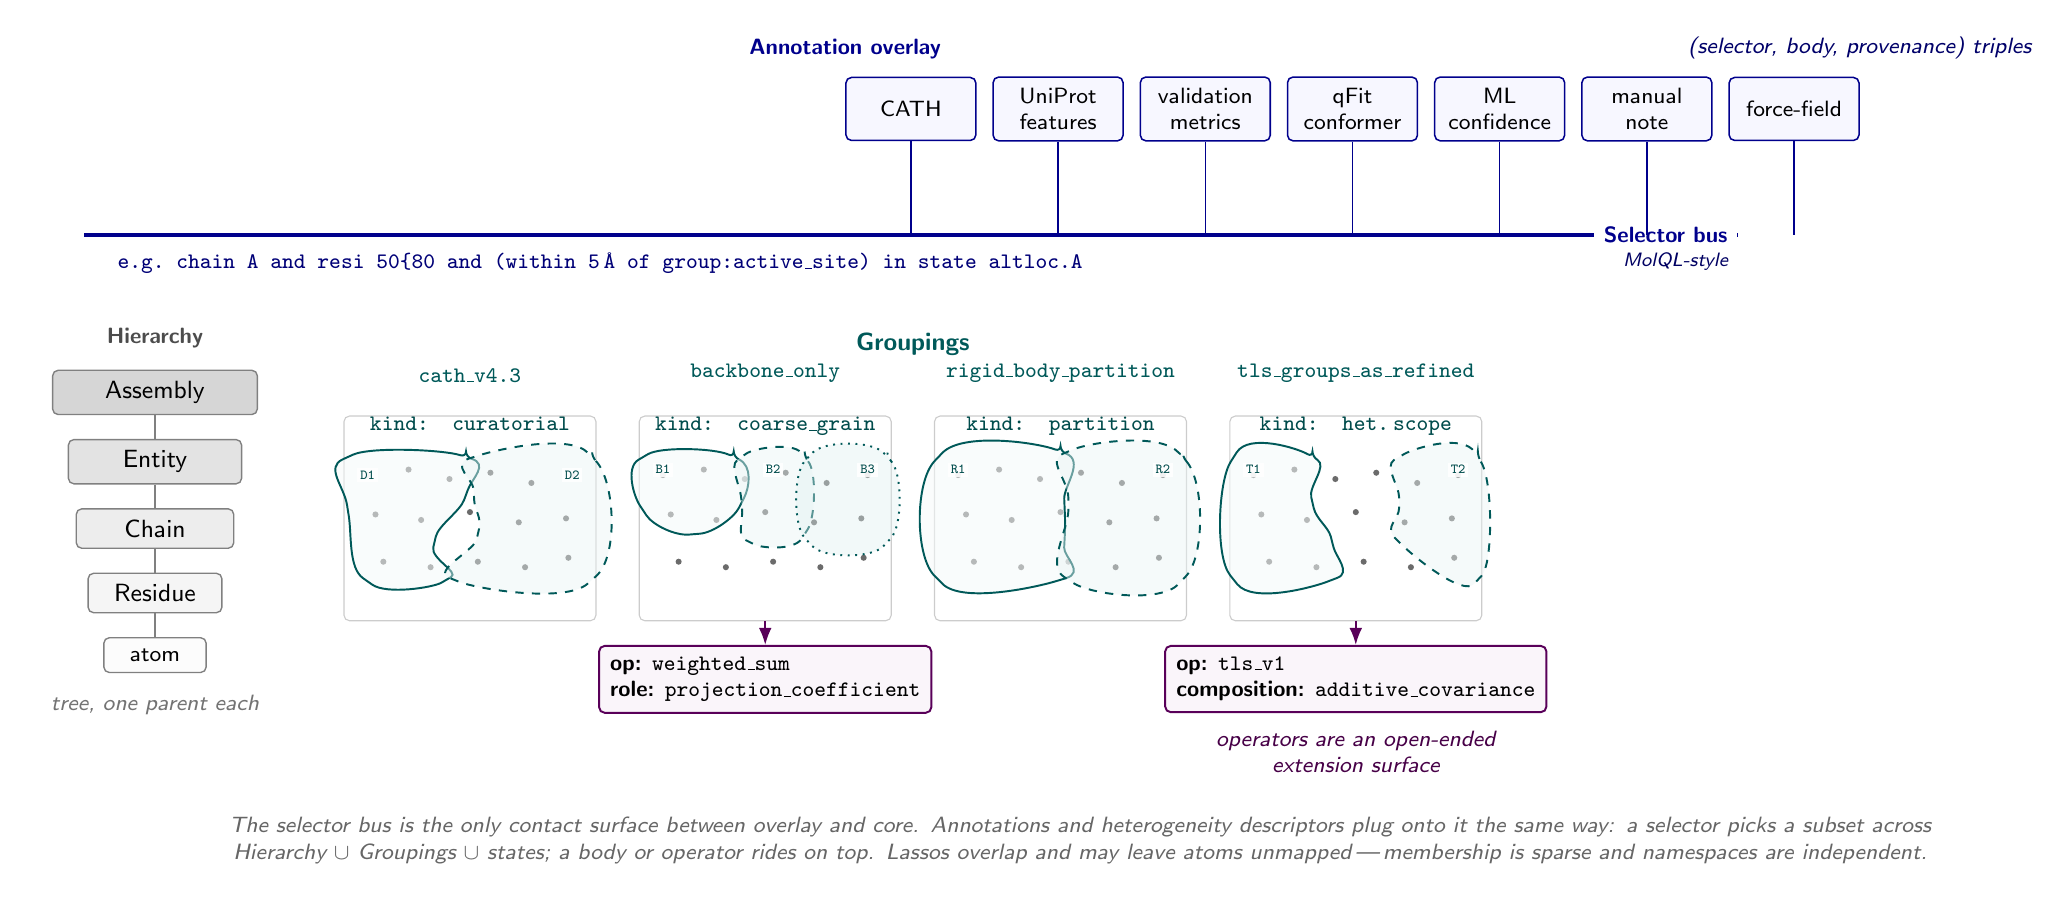
\begin{tikzpicture}

  % ============================================================
  % 1. Annotation overlay row
  % ============================================================
  \node[Lanno] (a1) at (0, 0) {CATH};
  \node[Lanno, right=2mm of a1] (a2) {UniProt\\features};
  \node[Lanno, right=2mm of a2] (a3) {validation\\metrics};
  \node[Lanno, right=2mm of a3] (a4) {qFit\\conformer};
  \node[Lanno, right=2mm of a4] (a5) {ML\\confidence};
  \node[Lanno, right=2mm of a5] (a6) {manual\\note};
  \node[Lanno, right=2mm of a6] (a7) {force-field};

  \node[font=\sffamily\footnotesize\bfseries, text=accA, anchor=south]
    at ($(a1.north west) + (0,1mm)$) {Annotation overlay};
  \node[font=\sffamily\footnotesize\itshape, text=accA!75!black, anchor=south]
    at ($(a7.north east) + (0,1mm)$)
    {(selector, body, provenance) triples};

  % ============================================================
  % 2. Selector bus  --  rendered as a thin rail rather than a slab
  % ============================================================
  % Bus rail: a thin horizontal line spanning the full core width.
  % Label sits on the right end; example query floats just below.
  \def\busY{-1.6}                  % y of the bus rail
  \coordinate (busL) at (-10.5, \busY);
  \coordinate (busR) at ( 10.5, \busY);
  \draw[accA, line width=1.2pt] (busL) -- (busR);

  % Bus label: a single small chip sitting on the right end of the rail
  \node[font=\sffamily\footnotesize\bfseries, text=accA, anchor=east,
        fill=white, inner sep=2pt]
    (busLabel) at (busR) {\,Selector bus\,};
  \node[font=\sffamily\scriptsize\itshape, text=accA!70!black,
        anchor=north east]
    at ($(busR) + (0,-1mm)$) {MolQL-style};

  % Example query: a single concise line below the rail
  \node[font=\sffamily\footnotesize\ttfamily, text=accA!85!black,
        anchor=north west]
    at ($(busL) + (0.3,-1mm)$)
    {e.g.\ chain A and resi 50\textendash 80
     and (within 5\,\AA{} of group:active\_site) in state altloc.A};

  % Vertical wires: each annotation drops to the rail
  \foreach \n in {a1,a2,a3,a4,a5,a6,a7} {
    \draw[annoWire] (\n.south) -- (\n.south |- busL);
  }

  % ============================================================
  % 3. CORE: Hierarchy (left) + Groupings 4 panels (right) + op cards
  % ============================================================
  % Layout coords (cm): bus is centered at x=0.
  % Hierarchy tree at left.   Groupings panels in 1x4 row to its right.
  % Operator cards in a row below, aligned to relevant panels.

  % --- Hierarchy: compact vertical tree on the left ---
  \def\hxleft{-9.6}
  \node[L0] (assembly) at (\hxleft, -3.6) {Assembly};
  \node[L1, below=3mm of assembly] (entity)   {Entity};
  \node[L2, below=3mm of entity]   (chain)    {Chain};
  \node[L3, below=3mm of chain]    (residue)  {Residue};
  \node[L4, below=3mm of residue]  (atom)     {atom};
  \draw[contain] (assembly) -- (entity);
  \draw[contain] (entity)   -- (chain);
  \draw[contain] (chain)    -- (residue);
  \draw[contain] (residue)  -- (atom);

  \node[font=\sffamily\footnotesize\bfseries, text=black!70, anchor=south]
    at ($(assembly.north) + (0,1.5mm)$) {Hierarchy};
  \node[font=\sffamily\footnotesize\itshape, text=black!55, anchor=north,
        align=center, text width=3.0cm]
    at ($(atom.south) + (0,-1.5mm)$) {tree, one parent each};

  % ============================================================
  % 4. Four grouping panels --- same cloud, different lassos
  % ============================================================
  % Cloud point coordinates (panel-local, origin at panel center):
  %    1  2  3  4  5  6        upper row (y near +0.55)
  %    7  8  9 10 11           middle row (y near 0)
  %   12 13 14 15 16           lower row  (y near -0.55)
  % Slight scatter for organic look.
  %
  % Panel size: 3.4cm wide (x-span +/-1.55), 2.0cm tall (y-span +/-0.85)
  %
  % Cloud point positions (panel-local), used for all 4 panels.
  \def\cloudpts{%
    1/-1.30/0.55, 2/-0.78/0.62, 3/-0.26/0.50,
    4/0.26/0.58,  5/0.78/0.45,  6/1.30/0.55,
    7/-1.20/0.05, 8/-0.62/-0.02, 9/0.00/0.08,
    10/0.62/-0.05, 11/1.22/0.00,
    12/-1.10/-0.55, 13/-0.50/-0.62, 14/0.10/-0.55,
    15/0.70/-0.62, 16/1.25/-0.50%
  }

  % Panel positions (centers). Y-row for the panels (clears bus + headers).
  \def\py{-5.2}
  \def\panW{3.4}
  \def\panGap{0.25}
  % Place 4 panels centered around x = +1.5
  \def\pxA{-5.6}    % panel 1 center x
  \def\pxB{-1.85}   % panel 2 center x
  \def\pxC{1.9}     % panel 3 center x
  \def\pxD{5.65}    % panel 4 center x

  % --- Panel 1: cath_v4.3 (curatorial) ---
  \node[panel] (P1) at (\pxA, \py) {};
  \foreach \i/\dx/\dy in \cloudpts {
    \node[cloud-dot] at ($(\pxA,\py) + (\dx,\dy)$) {};
  }

  % D1 lasso (solid, left chunk)
  \draw[lasso-A] plot[smooth cycle, tension=0.7] coordinates {
    ($(\pxA,\py) + (-1.55, 0.78)$)
    ($(\pxA,\py) + (-0.05, 0.78)$)
    ($(\pxA,\py) + (-0.05, 0.30)$)
    ($(\pxA,\py) + (-0.45,-0.30)$)
    ($(\pxA,\py) + (-0.30,-0.78)$)
    ($(\pxA,\py) + (-1.30,-0.80)$)
    ($(\pxA,\py) + (-1.55, 0.10)$)
  };
  \node[lassolbl] at ($(\pxA,\py) + (-1.30, 0.55)$) {D1};

  % D2 lasso (dashed, right chunk)
  \draw[lasso-B] plot[smooth cycle, tension=0.7] coordinates {
    ($(\pxA,\py) + (0.05, 0.78)$)
    ($(\pxA,\py) + (1.55, 0.78)$)
    ($(\pxA,\py) + (1.55,-0.78)$)
    ($(\pxA,\py) + (-0.20,-0.78)$)
    ($(\pxA,\py) + (0.10,-0.20)$)
    ($(\pxA,\py) + (0.05, 0.30)$)
  };
  \node[lassolbl] at ($(\pxA,\py) + (1.30, 0.55)$) {D2};

  % --- Panel 2: backbone_only (coarse_grain) ---
  \node[panel] (P2) at (\pxB, \py) {};
  \foreach \i/\dx/\dy in \cloudpts {
    \node[cloud-dot] at ($(\pxB,\py) + (\dx,\dy)$) {};
  }

  % B1 (solid)
  \draw[lasso-A] plot[smooth cycle, tension=0.7] coordinates {
    ($(\pxB,\py) + (-1.55, 0.78)$)
    ($(\pxB,\py) + (-0.40, 0.78)$)
    ($(\pxB,\py) + (-0.30, 0.20)$)
    ($(\pxB,\py) + (-0.90,-0.20)$)
    ($(\pxB,\py) + (-1.55, 0.10)$)
  };
  \node[lassolbl] at ($(\pxB,\py) + (-1.30, 0.62)$) {B1};

  % B2 (dashed)
  \draw[lasso-B] plot[smooth cycle, tension=0.7] coordinates {
    ($(\pxB,\py) + (-0.30, 0.78)$)
    ($(\pxB,\py) + ( 0.50, 0.78)$)
    ($(\pxB,\py) + ( 0.50,-0.20)$)
    ($(\pxB,\py) + (-0.20,-0.30)$)
    ($(\pxB,\py) + (-0.30, 0.20)$)
  };
  \node[lassolbl] at ($(\pxB,\py) + (0.10, 0.62)$) {B2};

  % B3 (dotted)
  \draw[lasso-C] plot[smooth cycle, tension=0.7] coordinates {
    ($(\pxB,\py) + (0.55, 0.78)$)
    ($(\pxB,\py) + (1.55, 0.78)$)
    ($(\pxB,\py) + (1.55,-0.30)$)
    ($(\pxB,\py) + (0.55,-0.30)$)
  };
  \node[lassolbl] at ($(\pxB,\py) + (1.30, 0.62)$) {B3};

  % Note: residues 12, 13, 14, 15 (lower row) are deliberately
  % outside any bead lasso -- bead assignment is sparse here.

  % --- Panel 3: rigid_body_partition (partition) ---
  \node[panel] (P3) at (\pxC, \py) {};
  \foreach \i/\dx/\dy in \cloudpts {
    \node[cloud-dot] at ($(\pxC,\py) + (\dx,\dy)$) {};
  }

  % R1 (solid, left half) -- partition: every dot in some R
  \draw[lasso-A] plot[smooth cycle, tension=0.7] coordinates {
    ($(\pxC,\py) + (-1.55, 0.78)$)
    ($(\pxC,\py) + ( 0.00, 0.85)$)
    ($(\pxC,\py) + ( 0.05, 0.18)$)
    ($(\pxC,\py) + ( 0.05,-0.30)$)
    ($(\pxC,\py) + ( 0.00,-0.78)$)
    ($(\pxC,\py) + (-1.55,-0.78)$)
  };
  \node[lassolbl] at ($(\pxC,\py) + (-1.30, 0.62)$) {R1};

  % R2 (dashed, right half)
  \draw[lasso-B] plot[smooth cycle, tension=0.7] coordinates {
    ($(\pxC,\py) + ( 0.10, 0.85)$)
    ($(\pxC,\py) + ( 1.55, 0.78)$)
    ($(\pxC,\py) + ( 1.55,-0.78)$)
    ($(\pxC,\py) + ( 0.10,-0.78)$)
    ($(\pxC,\py) + ( 0.10, 0.18)$)
  };
  \node[lassolbl] at ($(\pxC,\py) + (1.30, 0.62)$) {R2};

  % --- Panel 4: tls_groups_as_refined (heterogeneity_descriptor.scope) ---
  \node[panel] (P4) at (\pxD, \py) {};
  \foreach \i/\dx/\dy in \cloudpts {
    \node[cloud-dot] at ($(\pxD,\py) + (\dx,\dy)$) {};
  }

  % T1 (solid, left)
  \draw[lasso-A] plot[smooth cycle, tension=0.7] coordinates {
    ($(\pxD,\py) + (-1.55, 0.78)$)
    ($(\pxD,\py) + (-0.55, 0.78)$)
    ($(\pxD,\py) + (-0.55, 0.20)$)
    ($(\pxD,\py) + (-0.30,-0.30)$)
    ($(\pxD,\py) + (-0.30,-0.78)$)
    ($(\pxD,\py) + (-1.55,-0.78)$)
  };
  \node[lassolbl] at ($(\pxD,\py) + (-1.30, 0.62)$) {T1};

  % T2 (dashed, right)
  \draw[lasso-B] plot[smooth cycle, tension=0.7] coordinates {
    ($(\pxD,\py) + ( 0.55, 0.78)$)
    ($(\pxD,\py) + ( 1.55, 0.78)$)
    ($(\pxD,\py) + ( 1.55,-0.78)$)
    ($(\pxD,\py) + ( 0.55,-0.30)$)
    ($(\pxD,\py) + ( 0.55, 0.20)$)
  };
  \node[lassolbl] at ($(\pxD,\py) + (1.30, 0.62)$) {T2};

  % Note: a strip of dots in the middle of panel 4 is unmapped --
  % TLS partitions need not cover the whole structure.

  % --- Panel headers (above each panel) ---
  \node[panelhdr]  at ($(P1.north) + (0,3mm)$) {\texttt{cath\_v4.3}};
  \node[panelkind] at ($(P1.north) + (0,1.0mm)$) {kind: curatorial};

  \node[panelhdr]  at ($(P2.north) + (0,3mm)$) {\texttt{backbone\_only}};
  \node[panelkind] at ($(P2.north) + (0,1.0mm)$) {kind: coarse\_grain};

  \node[panelhdr]  at ($(P3.north) + (0,3mm)$) {\texttt{rigid\_body\_partition}};
  \node[panelkind] at ($(P3.north) + (0,1.0mm)$) {kind: partition};

  \node[panelhdr]  at ($(P4.north) + (0,3mm)$) {\texttt{tls\_groups\_as\_refined}};
  \node[panelkind] at ($(P4.north) + (0,1.0mm)$) {kind: het.\,scope};

  % --- "Groupings" header centered above the four panels ---
  \coordinate (GH) at ($(P1.north west)!0.5!(P4.north east) + (0,9mm)$);
  \node[font=\sffamily\small\bfseries, text=accG] at (GH) {Groupings};

  % (no central arrow; the rail itself is the bus visual)

  % ============================================================
  % 5. Operator detail column (only for panels that need it)
  % ============================================================
  \def\opy{-6.4}

  \node[Lop, anchor=north] (op2)
    at ($(P2.south) + (0,-3mm)$)
    {\textbf{op:} \texttt{weighted\_sum}\\
     \textbf{role:} \texttt{projection\_coefficient}};
  \draw[bind] (P2.south) -- (op2.north);

  \node[Lop, anchor=north] (op4)
    at ($(P4.south) + (0,-3mm)$)
    {\textbf{op:} \texttt{tls\_v1}\\
     \textbf{composition:} \texttt{additive\_covariance}};
  \draw[bind] (P4.south) -- (op4.north);

  \node[font=\sffamily\footnotesize\itshape, text=accO!80!black, anchor=north,
        align=center, text width=4cm]
    at ($(op4.south) + (0,-1mm)$)
    {operators are an open-ended\\extension surface};

  % ============================================================
  % 6. Subtle caption strip (below the operator cards)
  % ============================================================
  \node[font=\sffamily\footnotesize\itshape, text=black!60, align=center,
        text width=22cm, anchor=north]
    at ($(op4.south) + (-3.5cm,-12mm)$)
    {The selector bus is the only contact surface between overlay and core.
     Annotations and heterogeneity descriptors plug onto it the same way:
     a selector picks a subset across Hierarchy \(\cup\) Groupings \(\cup\) states;
     a body or operator rides on top.
     Lassos overlap and may leave atoms unmapped\,---\,membership is sparse
     and namespaces are independent.};

\end{tikzpicture}
\end{document}
